\documentclass[12pt,
	a4paper,
	listof=totoc,
	bibliography=totoc,
	parskip=full*
	]{scrreprt}

\usepackage[utf8x]{inputenc}
\usepackage[ngerman]{babel}
\usepackage[babel,german=quotes]{csquotes}
\usepackage[hidelinks]{hyperref}
\usepackage{amsmath}
\usepackage{paralist}
\usepackage{amsfonts}
\usepackage{amssymb}
\usepackage{caption}
\usepackage{pdfpages}
\usepackage{graphicx}
\usepackage{tabularx}
\usepackage{tabu}
\usepackage{enumerate}
\usepackage{adjustbox}
\usepackage[left=3.00cm, right=2.00cm, top=1cm, bottom=1.5cm,includeheadfoot]{geometry}
\usepackage{scrpage2}
\pagestyle{scrheadings}
\usepackage{todonotes}
\usepackage[toc,nonumberlist]{glossaries}
\usepackage{float}
\usepackage{wrapfig}
\usepackage{lscape}
\usepackage{rotating}
\usepackage{blindtext}

\renewcaptionname{ngerman}{\bibname}{Referenzen}

\newenvironment{uctab}{%
	\begin{minipage}{\textwidth}
	\captionsetup{type=table}
}{\end{minipage}\\*[6pt]}

% Glossar
\newglossaryentry{alkkalk}
{
  name=AlkKalk,
  description={Name unserer Anwendung. Setzt sich aus
			\underline{Alk}ohol \underline{Kalk}ulator zusammen}
}

\newglossaryentry{anwender}
{
  name=Anwender,
  description={Ist der Akteur, der AlkKalk auf seinem Android Smartphone benutzt.}
}

\newglossaryentry{applikation}
{
  name=Applikation,
  description={Anwendung}
}

\newglossaryentry{brainstorming}
{
  name=Brainstorming,
  description={Methode zur Ideenfindung, jede Idee wird
akzeptiert. Erst später werden sie gegeneinander abgewogen.}
}

\newglossaryentry{blutalkoholkonzentration}
{
  name=Blutalkoholkonzentration,
  description={Die Konzentration des Ethanols pro Liter Blut,
    wird üblicherweise in Promille angegeben.}
}

\newglossaryentry{materialdesign}
{
  name=Material Design,
  description={Material Design ist eine vom Unternehmen Google entwickelte Designsprache,
    die in Android verwendet wird.}
}

\newglossaryentry{metabolismus}
{
  name=Metabolismus,
  description={Stoffwechsel}
}

\newglossaryentry{persistent}
{
  name=Persistent,
  description={Persistent heisst, dass die Daten auch über die Laufzeit
    eines Programms hinaus gespeichert werden.}
}

\newglossaryentry{spezifikation}
{
  name=Spezifikation,
  description={Beschreibung des Produkts durch Auflistung seiner Anforderungen}
}

\newglossaryentry{userinterface}
{
  name=User Interface,
  description={Englisch für Benutzerschnittstelle,
    über welche der Anwender die Applikation steuern kann.}
}

\newglossaryentry{usability}
{
  name=Usability,
  description={Englisch für Benutzerfreundlichkeit}
}

\newglossaryentry{playstore}
{
  name=Google Play Store,
  description={Der Google Play Store ist ein App Store, der meist auf
    Smartphones und Tablet-Computern mit dem Betriebssystem Android ausgeliefert wird}
}

\newglossaryentry{getrank}
{
  name=Getränk,
  description={Ein Getränk ist ein Sammelbegriff für zum trinken zubereitete alkoholische Getränke. Alkoholische Getränke oder alkoholhaltige Getränke, auch Alkoholika oder (vor allem in Bezug auf Spirituosen) geistige Getränke genannt, sind Getränke, die Trinkalkohol (Ethanol) enthalten, der in Lebensmitteln meist nur als Alkohol bezeichnet wird.}
}


\newglossaryentry{kohasion}
{
  name=Kohäsion,
  description={Sollte möglichst stark sein und steht dafür,
    wie gut logische Einheiten durch \underline{eine} Programmeinheit umgesetzt wird}
}

\newglossaryentry{kopplung}
{
  name=Kopplung,
  description={Beschreibt das Mass der Verknüpfung zwischen Softwaremodulen.
    Das Ziel ist es, diese Abhängigkeit möglichst gering zu halten.}
}

\newglossaryentry{Wearables}
{
  name=Wearables,
  description={Wearables sind Tragbare Computersysteme, ein Beispiel hierfür wäre die IWatch von Apple.}
}




\makeglossaries

\newcommand{\mytitle}{PA HS16: Domänenübergreifende Sentiment-Analyse mit Deep Convolutional Neural Networks}
\newcommand{\myauthor}{Dirk von Grünigen, Martin Weilenmann}

\title{\mytitle}
\author{\myauthor}

\begin{document}
\begin{titlepage}
	
	\newcommand{\HRule}{\rule{\linewidth}{0.5mm}} % Defines a new command for the horizontal lines, change thickness here
	
	\center % Center everything on the page
	
	%----------------------------------------------------------------------------------------
	%	HEADING SECTIONS
	%----------------------------------------------------------------------------------------
	
	\textsc{\LARGE ZHAW}\\ % Name of your university/college
	\textsc{\Large Zürcher Hochschule für angewandte Wissenschaften}\\[1.0cm]
	\textsc{\Large Projektarbeit}\\[0.5cm] % Major heading such as course name
	\textsc{\large HS 2016}\\[0.5cm] % Minor heading such as course title
	
	%----------------------------------------------------------------------------------------
	%	TITLE SECTION
	%----------------------------------------------------------------------------------------
	
	\HRule \\[0.4cm]
	{ \huge \bfseries Domänenübergreifende Sentiment-Analyse mit Deep Convolutional Neural Networks}\\[0.4cm] % Title of your document
	\HRule \\[1.5cm]
	
	%----------------------------------------------------------------------------------------
	%	AUTHOR SECTION
	%----------------------------------------------------------------------------------------
	
	\begin{minipage}{0.4\textwidth}
		\begin{flushleft} \large
			\emph{Authoren:}\\
			Dirk \textsc{von Grünigen}\\
			Martin \textsc{Weilenmann}
		\end{flushleft}
	\end{minipage}
	~
	\begin{minipage}{0.4\textwidth}
		\begin{flushright} \large
			\emph{Betreuer:} \\
			Dr. Mark \textsc{Cielibak}\\
			Dr. Stephan \textsc{Neuhaus}\\
			Jan \textsc{Deriu}
		\end{flushright}
	\end{minipage}\\[2cm]
	
	% If you don't want a supervisor, uncomment the two lines below and remove the section above
	%\Large \emph{Author:}\\
	%John \textsc{Smith}\\[3cm] % Your name
	
	%----------------------------------------------------------------------------------------
	%	DATE SECTION
	%----------------------------------------------------------------------------------------
	
	{\large \today}\\[2cm] % Date, change the \today to a set date if you want to be precise
	
	%----------------------------------------------------------------------------------------
	%	LOGO SECTION
	%----------------------------------------------------------------------------------------
	
	
\includegraphics{img/logo_zhaw}\\[1cm] % Include a department/university logo - this will require the graphicx package
	
	%----------------------------------------------------------------------------------------
	
	\vfill % Fill the rest of the page with whitespace
	
\end{titlepage}

\chapter{Abstrakt}

ABSTRAKT

\newgeometry{top=0.75cm,bottom=1cm}
\tableofcontents
\restoregeometry

\chapter{Einführung}
\label{introduction}

Seit den frühen 2000er Jahren berfindet sich das stark Internet im Wandel: Aus einer grösstenteils statischen Sammlung von Informationen entwickelte sich im Lauf der Zeit eine dyamische, interaktive Plattform auf welcher Menschen aus der ganzen Welt Inhalte erstellen und teilen können. Dieser Wandel wurde durch das Aufkommen von sozialen Netzwerken, wie zum Beispiel Facebook oder Twitter, nochmals beschleunigt. Durch diese massive Flut an benutzererstellten Inhalten sind ganz neue Bedürfnisse entstanden, diese Inhalte automatisch zu analysieren \cite{Pang:2008}.\\\\
Bei der Sentiment Analyse geht es darum, einen ganzen Text oder einen einzelnen Satz nach desen Polarität, zum Beispiel positiv oder negative, zu klassifizieren. Diese Klassifizierung kann dazu verwendet werden die generelle Stimmung von Benutzer bezüglich eines Themas zu analysieren. Als Beispiel könnte man hier aufführen dass ein Filmproduzent überwachen und analysieren möchte wie gut sein neuster Film bei den Zuschauern, welche sich z.B. auf Twitter dazu äussern, ankommt.\\\\
Die menschliche Sprache enthält allerdings viele Konstrukte, welche es erschweren diese Aufgabe zu automatisieren. Dazu zählen Sprachkonstrukte wie Synonyme oder Homonyme, also Wörter welche gleich geschrieben werden aber eine andere Bedeutung haben (z.B. die Bank). Dann kommen noch sozialgesellschaftliche Phänomene wie Sarkasmus oder Zynismus, welche nur mit einem genügend grossen Kontextwissen richtig verstanden und interpretiert werden können.\\\\
Der Schwerpunkt dieser Arbeit liegt darin, zu analysieren, inwiefern sich Sentiment Analyse auf mehreren Domänen gleichzeitig durchführen lässt. Dafür bauen wir auf vorarbeiten von \cite{Deriu:2016} und \cite{Deriu:2016:MS} auf und verwenden das dort jeweils verwendete \emph{Convolutional Neural Network}.\\\\
In dieser Arbeit sollen die folgenden Forschungsfragen analysiert werden:\\
\begin{itemize}
	\item Lässt sich ein auf mehrere Domänen trainiertes Neuronales Netz, durch schritteweises Hinzufügen von Trainingsdaten der Zieldomäne, verbessern?
	\item Lässt sich ein bereits auf eine Zieldomäne trainiertes Neuronales Netz durch Hinzuziehen von weiteren Daten aus anderen Domänen, welche eine ähnliche Struktur aufweisen, verbessern?
	\item Inwiefern beeinflussen verschiedene Word Embeddings und die Distant-Phase \cite{Deriu:2016:MS} die Performanz des Systems?
\end{itemize}

Anmerkungen von Stephan Neuhaus:

\begin{itemize}

\item die haesslichen \verb+\\\\+ am Ende jedes Absatzes koennen Sie sich sparen, einfach eine Leerzeile einfuegen und es entsteht ein Absatz.

\item Sie sollten unbedingt lernen, wie man in \LaTeX{} Mathematik formatiert. Beispielsweise nimmt man nicht `\verb+*+', um Multiplikationen zu kennzeichnen, sondern laesst das Zeichen in der Regel einfach weg. Also nicht $a*b$, sondern einfach $ab$. Wenn man doch eins braucht, nimmt man einen Punkt, wie zb. $\mathbf{w} \cdot \mathbf{x}$ oder ein liegendes Kreuz, wie z.B. in $6.023\times10^{23}$. Der Stern ist reserviert z.B. fuer Konvolution: $(f*g)(x) = \int_a^x f(\xi)g(b-\xi) d\xi$.

\item Im Mathematikmodus funktioniert der Satz anders als im normalen Italic-Modus. Beispiel: \textit{flasche} (Italics) und $flasche$ (Mathematik). Wenn man Bezeichner im Mathe-Modus braucht, die mehr als einen Buchstaben lang sind, schliesst man die in \verb+\textit{...}+ ein: $\sin^2(2\textit{flasche} + 1)$. Die beiden letzte Punkte sollten Sie beruecksichtigen, wenn Sie Gl.~(\ref{basic:metrics:f1_eq}) neu setzen.

\item Ellipsen schreibt man nicht `\verb+...+', sondern `\verb+\dots+'. Hier der Unterschied: Mit Punkten ..., mit \verb+\dots+ \dots

\item Also an der Kommasetzung muessen Sie noch arbeiten.

\item Ich habe Abschnitt~\ref{basic:neural_network:neuron} mal umgeschrieben. Sie sollten sich abgewoehnen, Fuellwoerter wie "`essentiell"' oder "`im Grunde"' zu verwenden. Wenn etwas "`im Grunde"' so und so ist, dann ist es so und so, da braucht man "`im Grunde"' nicht. Sie sollten den umformulierten Abschnitt aber bloss als Anregung betrachten. Vielleicht halten Sie den alten und den neuen Abschnitt mal nebeneinander und schauen, was Ihnen besser gefaellt.

\item Einige der Umbenennungen in Abschnitt~\ref{basic:neural_network:neuron} habe ich vorgenommen, damit der Text besser auf das Bild passt; z.B. haben Sie von der Funktion $\gamma$ geschrieben, im Bild zu sehen war aber $\varphi$. Da muessen Sie aber noch den Schwellwert $\theta$ mit hineinbringen, damit es ganz passt.

\item Weil der rechte Rand so schmal ist, klappt das mit den Markierungen mit \verb+\fixme+ nicht so recht. Vielleicht sollten Sie bis zum endgueltigen Formatierungslauf breitere Raender in Betracht ziehen.

\item In Tabelle~\ref{basics:sentiments_example_table} habe ich die Defaults bei der Formatierung wiederhergestellt. Dazu gehoert, im \verb+tabular+-Environment auf die redundanten \verb+@{}+ zu verzichten und die Leerzeilen zu entfernen. Solche Defaults sind in der Regel sorgfaeltig ausgesucht und man veraendert diese auf eigene Gefahr.

\item Ich fand im Abschnitt ``Zero-Padding'' noch ein \verb+<<<<<<< HEAD+. Das habe ich mal entfernt :-)

\item Versuchen Sie, die Bildlegenden wo moeglich so zu gestalten, dass jemand, der nur die Bilder liest, zumindest eine Ahnung bekommt, was im Text vor sich geht. Ich habe das mal beispielhaft an Abbildung~\ref{fig:schichten} gemacht.

\item Mit Ihrer Abbildung~\ref{fig:schichten} scheint etwas nicht zu stimmen. Wenn ``HB'' fuer den \emph{H}idden \emph{B}ias stehen soll, zeigt der Bias auf das falsche Neuron; gleiches gilt fuer VB. (Wieso ueberhaupt ``V'' fuer die Eingabeschicht? Ich verstehe ``H'' fuer ``Hidden'', aber nicht ``V''.) Ausserdem ist mir nicht klar, wieso alle Neuronen einer Schicht dasselbe Bias haben sollten.

\end{itemize}

\chapter{Grundlagen}
Im ersten Teil dieses Kapitels werden die theoretischen Grundlagen, welche in den folgenden Kapitel dieser Arbeit Verwendung finden, erläutert. Dabei werden zuerst grundlegende Begriffe wie Sentiment und Domäne eingeführt. Danach folgt eine Einführung in das maschinelle Lernen mit Neuronalen Netzwerken sowie einer speziellen Variante, dem sogenannten \gls{cnn}. Zu guter Letzt wird das 3-stufige Lernverfahren, mit welchem die zuvor genannten Netzwerke trainiert werden, erläutert.

Die folgenden Erläuterungen müssen im Kontext von Sentiment-Analyse beachtet werden. Sentiment-Analyse ist ein Klassifizierungsproblem. Natürlich lassen sich Neuronale Netze auch für weitere Aufgaben (z.B. Dimensionalitätsreduktion, Vorraussagen von Werten) einsetzen, allerdings werden diese Themen in den folgenden Äusserungen nicht mit einbezogen.

\section{Definitionen}
\paragraph{Sentiment}
Der \emph{Sentiment} beschreibt das subjektive Empfinden welches beim Leser eines Textes ausgelöst wird. Ein Sentiment kann für einzelne Sätze, Abschnitte oder ganze Texte bestimmt werden. Im Rahmen dieser Arbeit werden die drei Sentiments \emph{positiv}, \emph{neutral} und \emph{negativ} verwendet (vgl. Beispiele in Tabelle \ref{basics:sentiments_example_table}). Je nach Bedürfnis lässt sich diese Skala noch weiter verfeinern (z.B. mit emph{eher negativ} oder \emph{eher positiv} als Sentiments).

\begin{table}[h]
  \centering
  \begin{tabular}{ll}
    \toprule
    Sentiment & Beispiel\\
    \midrule
    positiv & Ich liebe Donuts!\\
    neutral & Dieser Stein ist grau.\\
    negativ & Die Auflösung dieser Handy-Kamera ist sehr schlecht.\\
    \bottomrule
  \end{tabular}
  \caption{Beispieltexte für die drei verschiedenen Sentiments}
  \label{basics:sentiments_example_table}
\end{table}

Der Sentiment eines Textes ist nicht eindeutig bestimmt, da dieser vom subjektiven Empfinden der annotierenden Person bestimmt wird. Je nachdem wer den Sentiment eines Textes bestimmt kann ein anderes Ergebnis zur Folge haben.
Da der Sentiment eines Textes nach dem subjektiven Empfinden einer Person bestimmt wird ist dieser nicht eindeutig. Je nachdem wer einen Text beurteilt kann also ein anderes Ergebnis zur Folge haben.

\paragraph{Domäne} Texte, welche die gleiche Struktur aufweisen werden zu einer Domäne zusammengefasst. Als Beispiele lassen sich hier Produktbewertungen, Tweets oder auch Nachrichtentexte erwähnen.\fixme{Besser beschreiben!}

\paragraph{Crossdomain} 
Mit \emph{Crossdomain} (dt. domänenübergreifend) ist die Verwendung von Trainings- und Testdaten aus mehreren verschiedenen Domänen zum Training und/oder zur Validierung eines Sentiment-Klassifiziers gemeint.

\paragraph{Formale Definitionen}

Für die Durchführung dieser Arbeit sind keine formale Definitionen der zuvor genannten Begriffe nötig. Solche können allerdings in diversen anderen Arbeiten, unter anderem \ref{...} und \ref{...}, gefunden werden.

\section{Neuronale Netzwerke}
\label{basics:neural_network}

Neuronale Netzwerke, im Folgenden \emph{\gls{NN}} genannt, sind ein Modell des maschinellen Lernens, welches biologisch motiviert ist und sich lose an der Struktur menschlichen Gehirn orientiert. Im folgenden wird auf die einzelnen Komponenten eines NN eingegangen.

\paragraph{Neuron}\label{basic:neural_network:neuron} Ein NN besteht aus \emph{Neuronen}, manchmal auch Perceptronen genannt. Diese bilden einen mathematische Funktion ab und sind die Grundbausteine eines NN.

Diese Neuronen nehmen $n$ Eingangswerte $\mathbf{x} = (x_0, x_1, \dots, x_n)$ entgegen. Jedem dieser Eingangswerte $x_n$ wird ein Gewicht $w_n$ aus der Menge $\mathbf{w} = (w_0, w_1, \dots, w_n)$ zugewiesen. Der Eingangswert $x_0$ bzw. das zugehörige Gewicht $w_0$ werden fast immer auf $1$ gesetzt und als Bias-Wert bzw. -Gewicht bezeichnet. Mithilfe der Eingangswerte $\mathbf{x}$, den zugehörigen Gewichten $\mathbf{w}$ und der Aktivierungsfunktion $\varphi$ wird die Ausgabe $o$, auch Aktivierung genannt, des Neurons wie folgt berechnet:
\begin{equation}
o = \varphi(\mathbf{w} \cdot \mathbf{x}) = \varphi\bigg(\sum_{i=0}^{n} w_i x_i\bigg)
\label{basics:neural_network:compute_equation}
\end{equation}
Die Aktivierungsfunktion $\varphi$ ist dafür zuständig den aus der Berechnung resultierenden Wert $o$ in eine vordefinierte Spanne von Werten zu bringen. Beispiele für häufig verwendete Aktivierungsfunktionen sind $\tanh(x) = (e^x - e^{-x})/(e^x + e^{-x})$, $\operatorname{relu}(x) = \max\{0,x\}$ oder die sigmoid-Funktion $s(x) = 1/(1 + e^{-x})$.

Im Rahmen dieser Arbeit wird ausschliesslich $\operatorname{relu}$ als Aktivierungsfunktion verwendet.

\paragraph{Schicht}\label{basic:neural_network:layer} Mithilfe der zuvor erwähnten Neuronen werden die einzelnen Schichten eines NN aufgebaut. Eine Schicht setzt sich dabei aus mehreren Neuronen zusammen. Um ein vollständiges NN zu erhalten werden mehrere dieser Schichten hintereinander gereiht. Dabei gibt es drei essentielle Schichten, welches fast jedes neuronale Netzwerk (im klassischen Sinne) hat: Eine \emph{Eingabeschicht}, eine oder mehrere \emph{Hiddenschichten} oder \emph{verborgene Schichten} und eine \emph{Ausgabeschicht}; vgl.\ Abbildung~\ref{fig:schichten}.

\begin{figure}[h]
  \centering
  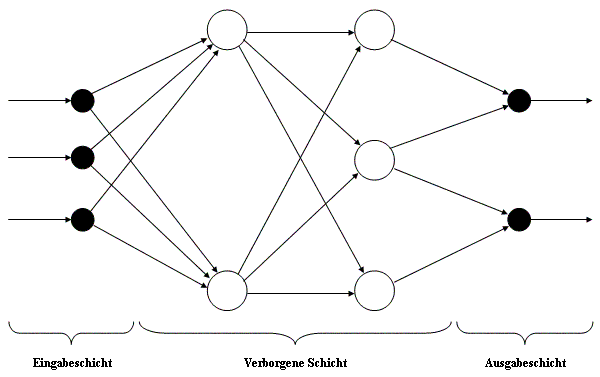
\includegraphics[width=10cm]{img/basic_neural_network}
  \caption{Schematische Darstellung eines neuronalen Netzwerkes. Links die Eingabeschicht, in der Mitte eine Hiddenschicht, rechts die Ausgabeschicht.}
  \label{fig:schichten}
\end{figure}

Über die Eingabeschicht treten die Eingabedaten $\mathbf{x} = (x_1, x_2, \dots, x_n)$ in das Netzwerk ein. Diese werden dann an die Neuronen der Hiddenschicht vorwärtspropagiert und diese berechnen damit ihre Aktivierungen $o_{11}, o_{12}, \dots, o_{1n}$. Die Aktivierungen werden dann von der Hiddenschicht zur Ausgabeschicht weitergereicht wo die sich darin enthaltenen Neuronen wiederum ihre Aktivierungen $o_{21}, o_{22}, \dots, o_{2n}$ berechnen. Die Eingabewerte der einzelnen Neuronen der Ausgabeschicht sind dabei die Aktivierungen aller Neuronen der vorhergehenden Schicht. Eine solche Schicht wird auch als \emph{fully-connected} Schicht bezeichnet, da die Eingabewerte jedes Neurons die Aktivierung aller Neuronen in der vorhergehenden Schicht sind.

Dieser Vorgang des "Vorwärtsrechnens" wird auch als Vorwärtspropagierung bezeichnet. Bei einem NN mit mehr als einer Hiddenschicht spricht man auch von einem \emph{Deep Neural Network}. Die Anzahl der Schichten und Neuronen in einem NN hängt stark von der konkreten Problemstellung ab.

\paragraph{Backpropagation mit Gradient-Descent} Wie bei fast allen Modellen des maschinellen Lernens lernt das NN mittels dem Optimieren einer Fehlerfunktion $E$. Als Fehlerfunktion kann jede Funktion dienen, mit welcher der Aussagefehler des Netzwerks quanitifiziert werden kann. Als Beispiele können hier der \emph{Mean Squared Error} $\operatorname{MSE}(y_{true}, y_{pred}) = \frac{1}{n}\sum_{i=0}^{n} (y_{pred} - y_{true})^2$ oder auch die in dieser Arbeit verwendete Categorical Cross-Entropy \fixme{Formula?} aufgeführt werden. Das Optimieren dieser Fehlerfunktion wird meistens mittels dem \emph{Backpropagation}-Algorithmus in Verbindung mit \emph{Gradient-Descent} durchgeführt. Der Algorithmus kann in folgenden Schritten zusammengefasst werden:

\begin{enumerate}
  \item Die Eingabewerte in das NN einführen und die Vorwärtspropagierung durchführen.
  \item Die Ausgabewerte des NN werden mit dem erwarteten Resultat verglichen. Die Differenz der Ausgabewerte von den erwarteten Werten wird als Aussagefehler des NN bezeichnet.
  \item Der Aussagefehler wird nun durch das NN hindurch zurückpropagiert. Dabei werden die Gewichte der einzelnen Schichten abhängig von ihrem Einfluss auf die berechneten Ausgangswerte verändert.
\end{enumerate}

Die Berechnung des Einfluss eines einzelnen Gewichtes wird mittels der partiellen Ableitung der Fehlerfunktion $E$ bezüglich dem entsprechenden Gewicht festgestellt. Danach wird das Gewicht neu berechnet indem der Wert der partiellen Ableitung multipliziert mit der Lernrate $\eta$ vom aktuellen Gewicht subtrahiert. Die Lernrate gibt dabei an wie stark sich ein einzelner Durchlauf von Backpropagation auf die Gewichte auswirken soll. Das neue Gewicht für das Neuron $i$ in der Schicht $k$ berechnet sich bei gegebener Lernrate $\eta$ und Fehlerfunktion $E$ also wie folgt:

\begin{equation}
w_{ik} = w_{ik} - \eta \frac{\delta E}{\delta w_{ik}}
\end{equation}

Gradient-Descent besitzt das Problem, dass der Erfolg des Algorithmus stark von der gewählten Lernrate $\eta$ abhängt. Bei einer zu grossen Lernrate wird das Optimum möglicherweise übersprungen oder der Wert der Fehlerfunktion divergiert sogar; bei einer zu kleinen Lernrate dauert es sehr lange bis das Optimum der Fehlerfunktion gefunden wird (vgl. Abbildung~\ref{fig:learn_rates}). Darum wird im Rahmen dieser Arbeit die weiterentwickelte Variante \emph{AdaDelta} \cite{zeiler2012adadelta} verwendet. Diese hat den grossen Vorteil das keine Lernrate mehr definiert werden muss.

\begin{figure}[h]
  \centering
  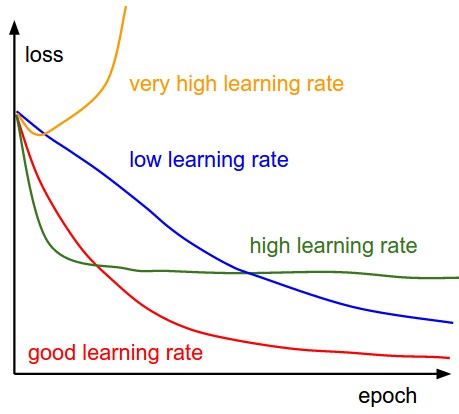
\includegraphics[width=6cm]{img/learning_rates_comparison}
  \caption{Beispielhafte gegenüberstellung verschiedener Lernraten\protect\footnote{http://cs231n.github.io/assets/nn3/learningrates.jpeg}}
  \label{fig:learn_rates}
\end{figure}

\section{Convolutional Neural Network}
\emph{Convolutional Neural Networks}, im Folgenden \gls{CNN} genannt, sind eine spezielle Form der zuvor beschriebenen NN. Der grundlegende Unterschied besteht darin, dass die einzelnen Schichten nicht fully-conntected sind, sondern mittels Filter über lokale Konnektivität versucht wird Muster zu erkennen. Im folgenden werden die einzelnen Komponenten des in dieser Arbeit verwendeten CNNs erläutert.

\paragraph{Filter}\label{basic:cnn:filter} Anstatt Neuronen wie im klassischen Neuronalen Netzwerk lernt eine CNN über die sogenannten Filter. Dabei handelt es sich um $n\times m$-Matrizen, welche Gewichte enthalten, analog zu den Gewichten der eingehenden Verbindungen bei Neuronen. Dabei werden die Filter-Matrizen über die Eingabedaten bewegt und es wird jeweils das innere Produkt der aktuellen Filter-Matrix und dem aktuellen Ausschnitt der Eingabedaten berechnet auf welchem der Filter positioniert ist. Das Bewegungsmuster des Filters wird \emph{Stride} (dt. durchschreiten) genannt. Im Rahmen dieser Arbeit wird nur ein eindimensionaler Stride entlang der Satz-Matrix (vgl. \ref{missing!}) verwendet.

Die durch diese Convolution-Operation resultierende Werte werden der Form einer Resultat-Matrix, der sogenannten \emph{Feature Map}, zwischengespeichert. Diese stellen also das Äquivalent zur Aktivierung einer Schicht im klassischen Neuronalen Netzwerk dar. Dabei werden alle resultierenden Feature-Maps einfach hintereinandergereiht und dienen als Eingabewerte für die nächste Schicht. 

\begin{figure}[h]
	\centering
	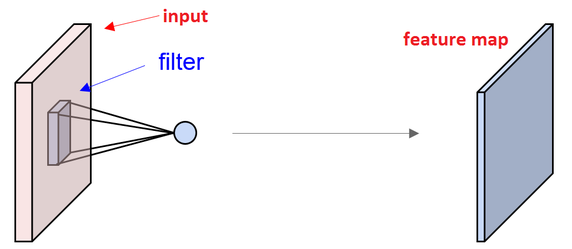
\includegraphics[width=10cm]{img/filter_feature_map}
	\caption{Schematische Darstellung Filter und Feature-Map}
\end{figure}

Eine Schicht, welche diese Art von Berechnung verwendet wird auch Convolutional (dt. sich falltend) Schicht genannt.

\paragraph{Max-Pooling Schicht} In der \emph{Max-Pooling} Schicht wird ein grossteil der in den Feature-Maps vorhandenen Informationen verworfen. Dabei wird ein Fenster über die resultierenden Feature-Maps der vorhergehenden Schicht bewegt und der jeweils maximale Wert des entsprechenden Ausschnitts der aktuellen Feature-Map als Wert in die gepoolte Represäntation übernommen. Das Fenster, welches über die Feature-Map bewegt wird, ist definiert durch die Dimensionalität des Fensters und dem Stride. Der Stride steht für das Bewegunsmuster des Fenster analog zum Filter. Die gepoolten Represäntationen der Feature-Maps dienen dann als Eingabewerte für die nächste Convolutional oder Ausgabeschicht.

\begin{figure}[H]
	\centering
	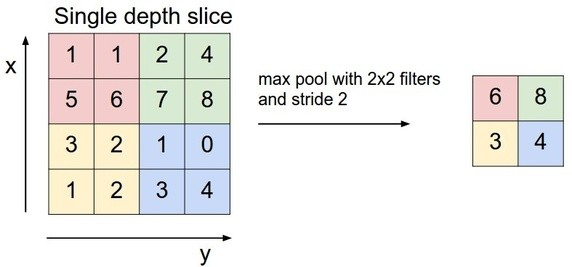
\includegraphics[width=10cm]{img/max_pooling}
	\caption{Schematische Funktionsweise der Max-Pooling Schicht}
\end{figure}

Die Max-Pooling Schicht erfüllt zwei Aufgaben: Einerseits reduziert sie die Dimensionalität der zu verarbeitenden Daten, andererseits verwirft sie \quotes{unwichtige} Informationen indem sie nur die maximalen Werte der zuletzt berechneten Aktivierungen behält.\fixme{more infos?}

\paragraph{Convolutional+Max-Pooling Schicht} Die Convolutional und Max-Pooling Schicht bilden die Grundbausteine des CNN. Diese werden nun mehrfach hintereinander gereiht. Das im Rahmen dieser Arbeit vewendete CNN hat bespielsweise zwei solcher aufeinanderfolgenden Convolutional+Max-Pooling Schichten.

\begin{figure}[h]
	\centering
	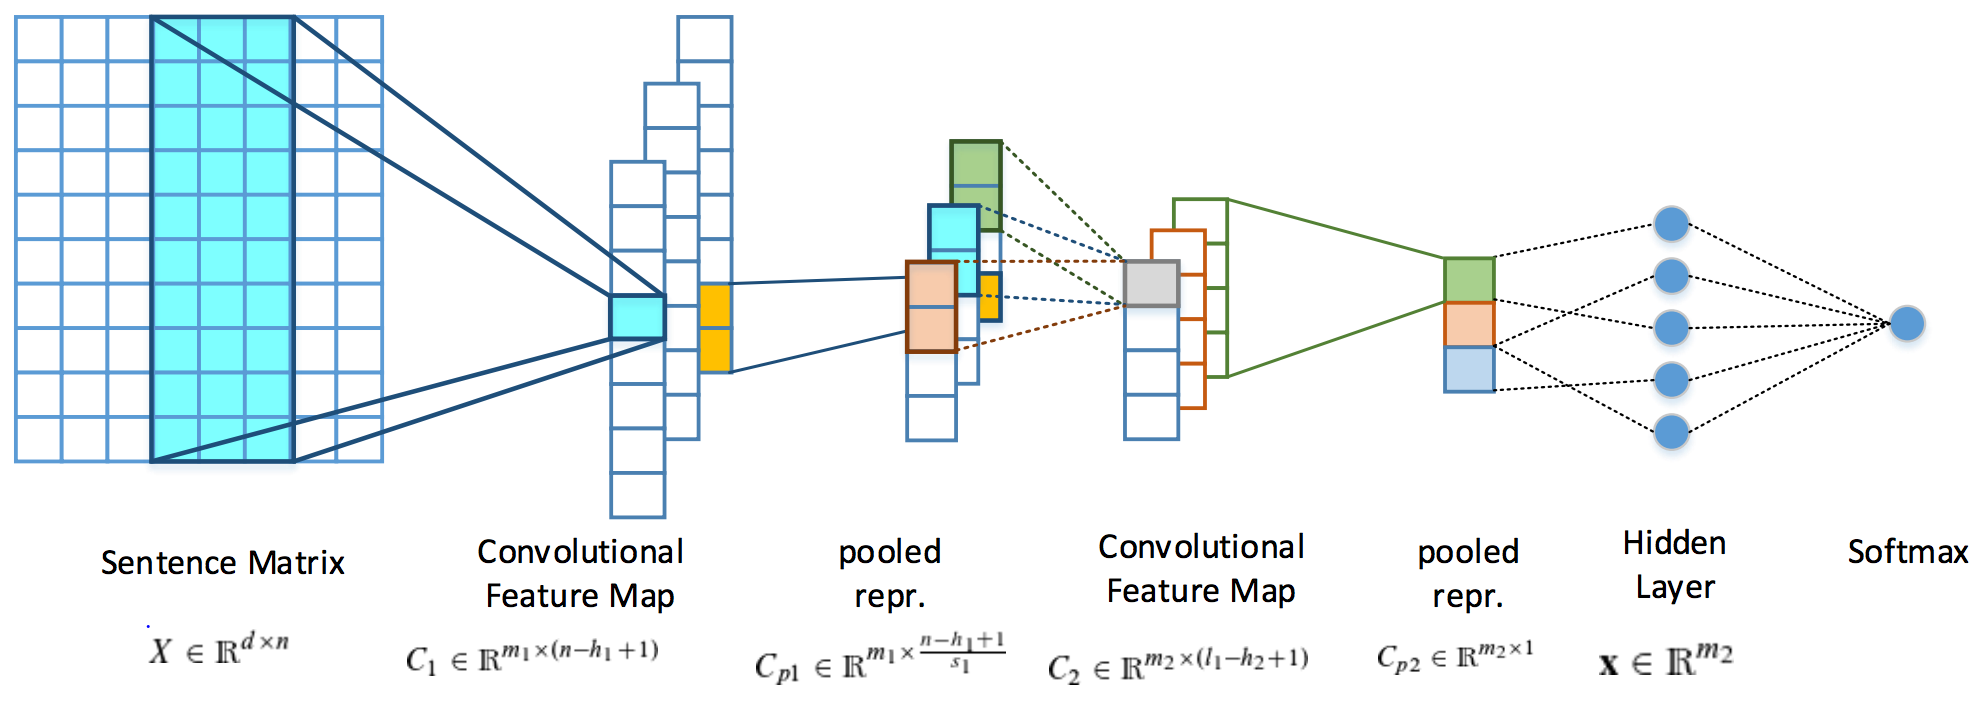
\includegraphics[width=10cm]{img/semeval_cnn_structure}
	\caption{Schematische Darstellung des in dieser Arbeit verwendeten CNN \protect\cite{deriu2016swisscheese}}
\end{figure}

\paragraph{Ausgabeschicht}\label{basic:cnn:output_layer} Die Ausgabeschicht des CNN ist gleich aufgebaut wie die eines \quotes{traditionellen} Neuronalen Netzwerks. Dabei wird eine fully-connected Schicht verwendet bei welcher alle Neuronen als Eingabewerte alle Aktivierungen der letzten Max-Pooling Schicht verknüpft sind. Die Anzahl Neuronen in der Ausgabeschicht entspricht dabei der Anzahl zu unterscheidenden Klassen.

\section{3-Phasen Lernen}

Das Training des CNNs wird mithilfe des 3-stufigen Lernverfahren von Severyn et. al. \cite{Severyn:2015kta} durchgeführt. Im Folgenden werden die einzelnen Schritte im Detail erläutert.

\paragraph{Word-Embeddings und Satz-Matrix} Zuerst werden mithilfe von \emph{word2vec}~\cite{mikolov2013distributed} und einem grossen Text-Corpus Word-Embeddings generiert. Dabei werden die gegebenen Wörter eines Vokabulars $v$ so in einen reelen Vektorraum $\mathbb{R}^d$ abgebildet, dass die semantischen Beziehungen innerhalb der Wörter erhalten bleiben. Dies wird am Beispiel in Abbildung \ref{fig:king_queen_example} ersichtlich: Die Wortvektoren für \quotes{Man} and \quotes{Woman} stehen in gleicher Weise zueinander wie die Wortvektoren \quotes{Uncle} zu \quotes{Aunt} bzw. \quotes{King} zu \quotes{Queen}.

\begin{figure}[H]
  \label{fig:king_queen_example}
  \centering
  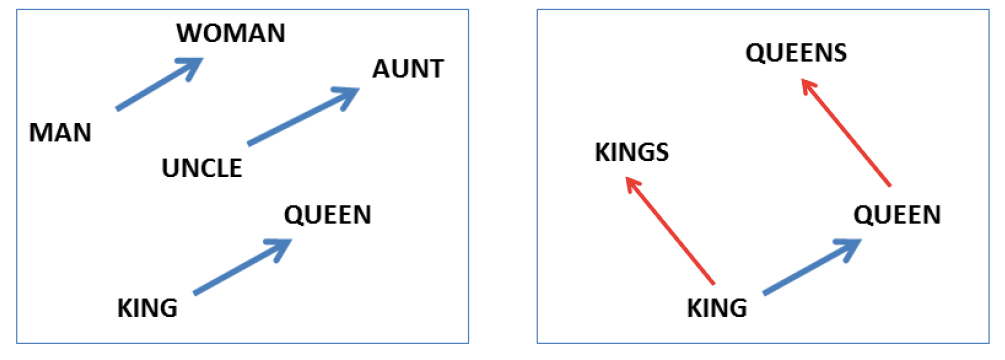
\includegraphics[width=10cm]{img/king_queen_example_word_embeddings}
  \caption{Beispiel für semantische Beziehung von Wort-Vektoren}
\end{figure}

Mithilfe der Word-Embeddings kann ein gegebener Satz nun als Konkatenation der Vektoren der einzelnen Wörter aufgefasst werden. Das bedeutet, dass ein Satz als $d \times n$ Matrix dargestellt werden kann, wenn $n$ die Anzahl Wörter des Satzes darstellt und $d$ die Anzahl Dimensionen der Word-Embeddings. Die $i$-te Zeile in der resultierenden Satz-Matrix entspricht dann dem Wort-Vektor für das $i$-te Wort im abzubildenden Satz.

\paragraph{Distant-Supervision Phase} In einem zweiten Schritt wird die sogenannte \emph{Distant-Supervised} Phase durchgeführt. Dabei wird das CNN mit einer grossen Menge an \emph{weakly-labeled} (dt. schwach annotiert) Texten über eine Epoche hinweg vortrainiert. Weakly labeled bedeutet, dass der Sentiment eines Textes aus der Eigenschaft des Textes abgeleitet wird und nicht von Hand annotiert wurde. Beispiele für Eigenschaften, aus welchen sich ein Sentiment ableiten lässt sind Emoticons in Tweets oder die Anzahl der vergebenen Sterne bei einer Produktbewertung. Bei Emoticons lässt sich zum Beispiel aus dem lachenden Emoticon \quotes{:-)} ein positiver bzw. aus dem traurigen Emoticon \quotes{:-(} ein negativer Sentiment ableiten.

\paragraph{Supervised Phase} Im letzten Schritt wird das CNN mit den von Hand annotierten Texten trainiert. Dieses Training wird mithilfe von Backpropagation mit AdaDelta durchgeführt. Dabei wird sogenanntes \emph{Early Stopping} verwendet: Das Netzwerk wird solange trainiert, bis eine definierte Metrik über eine bestimmte Anzahl Epochen nicht mehr verbessert hat.

\section{Evaluierungsmetrik}
Im folgenden wird die verwendete Evaluierungsmetrik, der \emph{F1-Score}, erläutert.

\paragraph{Precision {\&} Recall} \emph{Precision} (dt. Präzision) und \emph{Recall} (dt. Ausbeute) sind Metriken, mit welchen die Performanz eines Systems evaluiert werden kann. Dabei ist die Precision das Verhältnis von richtig klassifizierten ($\textit{tp}$) zu allen klassifizierten Samples ($\textit{tp} + \textit{fp}$):
\begin{equation}
\textit{precision} = \frac{\textit{tp}}{\textit{tp} + \textit{fp}}
\end{equation}
Die Ausbeute ist das Verhältnis von richtig klassifizierten zur Anzahl aller vorhandenen Samples ($\textit{tp} + \textit{fn}$):
\begin{equation}
recall = \frac{\textit{tp}}{\textit{tp} + \textit{fn}}
\end{equation}
Mit diesen beiden Metriken kann die Performanz eines Systems bewertet werden, allerdings haben diese zwei Nachteile: Einerseits sind es zwei einzelne Werte anstatt eines einzelnenen Wertes. Dies macht die Beurteilung über die Performanz des Systems komplizierter. Ausserdem kann mittels \quotes{schummeln} eine sehr hohe Ausbeute erreicht werden, indem nämlich immer nur eine bestimmte Klasse zurückgegeben wird.
\paragraph{F1-Score} Um da oben beschriebene Problem zu lösen wird der F1-Score verwendet. Dieser ist das harmonische Mittel von Präzision und Ausbeute:
\begin{equation}
\label{basic:metrics:f1_eq}
F1 = \frac{2 \times \textit{precision} \times recall}{\textit{precision} + \textit{recall}}
\end{equation}
Durch diese Metrik kann die Performanz eines Systems mittels eines Wertes quantifiziert werden. Ausserdem löst diese das Problem, dass eine hohe Präzision bzw. Ausbeute erzielt werden kann, wenn das System \quotes{schummelt} indem dieses immer die am stärksten vertretene Klasse als Antwort liefert.
\paragraph{F1-Score über mehrere Klassen} Der F1-Score selbst kann nur jeweils für eine einzelne Klasse bestimmt werden. Um nun aber eine einzige Metrik für die Messung der Performanz des Systems über mehrere Klassen hinweg zu erhalten, werden die F1-Scores der einzelnen Klassen summiert und durch die Anzahl der Klassen dividiert. Durch diese Vorgehen erhält man folgende Gleichung, wobei $k_i$ für eine einzelnen Klasse und $n$ für die Anzahl der beachteten Klassen:
\begin{equation}
\operatorname{F1}_{k_0, k_1, \dots, k_n} = \frac{\sum_{i=0}^{n} \operatorname{F1}_{k_i}}{n}
\end{equation}
Diese Art des F1-Score über mehrere Klassen hinweg wird auch \emph{macro-average} F1-Score genannt.

\section{Technischer Aufbau}
Im folgenden Abschnitt wird der technische Aufbau, welcher implementiert wurde, um die in \ref{experiments} beschriebenen Experimente durchzuführen. Eine genaue Beschreibung der Funktionsweise und Verwendung des Systems befindet sich in Anhang \ref{appendix:software_usage}.

\subsection{Vorarbeiten}
\label{technichal_setup:prework}
Der Grundaufbau der verwendeten Software wurde vom InIT mithilfe von Keras\footnote{https://keras.io/} implementiert und zur Durchführung dieser Arbeit zur Verfügung gestellt. Im Rahmen dieses Grundaufbaus wurde die folgende Funktionalität bereits implementiert:

\begin{itemize}[noitemsep]
	\item Implementation des CNN in Keras und verwendung von Theano \cite{theanoCitShort} als Backend für die \gls{GPU}s (vgl. Abschnitt \ref{technichal_setup:hardware}).
	\item Implementation von Evaluations-Metriken
	\item Skripte mit den folgenden Funktionalitäten: Trainieren des CNN, Laden von TSV Dateien, Vorverarbeiten von Word-Embeddings
\end{itemize}

\subsection{Anforderungen}
\label{technical_setup:requirements}
Ein System, welches die in \ref{experiments} beschriebenen Experimente durchführen kann, soll die folgenden Eigenschaften aufweisen:

\begin{itemize}
	\item \textbf{Parametrisierbarkeit}: Dadurch dass eine grosse Anzahl kleiner Experimente durchgeführt werden muss soll das System die Möglichkeit bitten Experimente parametrisiert durchzuführen.
	\item \textbf{Wiederholbarkeit}: Experimente sollen wenn nötig mehrfach durchgeführt werden ohne einen Mehraufwand zu verursachen. 
	\item \textbf{Übersichtlichkeit}: Resultate der Experimente sollen übersichtlich und einfach zugänglich sein.
	\item \textbf{Auswertbarkeit}: Resultate sollen \fixme{Bessers Wort für Einfach?} einfach ausgewertet werden können.
\end{itemize}

Die in \ref{technichal_setup:prework} beschriebenen Vorarbeiten bitten eine Basis um damit ein System aufzubauen, welches die oben beschriebenen Eigenschaften aufweist.
\subsection{Funktionalität}
\label{technical_setup:functionality}
Um ein System, welches die im vorhergehenden Kapitel beschriebenen Eigenschaften aufweist, zu erhalten, wurden die folgenden Komponenten implementiert:

\begin{itemize}
	\item \textbf{Executor}: Der \emph{Executor} ist zuständig für das Training der CNNs mithilfe von Keras. Beim Start akzeptiert er die Konfiguration als Parameter. Das Experiment wird mit dem Laden der benötigten Daten und dem anschliessenden Training des CNN gestartet. Am Ende jeder Epoche wird das aktuelle CNN auf den Validierungsdaten getestet und die konfigurierten Metriken ausgewertet. Diese werden am Ende zusammen mit dem trainierten CNN (Gewichte im HDF5-Format\footnote{https://support.hdfgroup.org/HDF5/}, das CNN Model als JSON) in einen für das Experiment vorgesehenen Ordner gespeichert. Die Metriken werden ebenfalls in diesem dem dafür vorgesehenen Ordner abgespeichert.
	\item \textbf{Config Management}: Experimente werden über Konfigurationen im JSON-Format\footnote{http://www.json.org/} parametrisiert. Über diese Konfiguration können viele wichtige Parameter für die Ausführung festgelegt werden, so zum Beispiel: Anzahl Epochen, Trainings- und Validierungsdaten, Parameter für k-fold Cross-Validation oder auch bereits Trainierte Modelle können geladen werden. Für eine vollständige Liste wird auf den Quellcode des Projektes verwiesen. Experimente können mittels der group{\_}id gruppiert werden. Damit können die Experimente hierarchisch mittels zwei Ebenen gruppiert werden.
	\item \textbf{DataLoader}: Mithilfe des \emph{DataLoader} können Trainings- und Validierungsdaten im TSV\footnote{https://reference.wolfram.com/language/ref/format/TSV.html} Dateiformat geladen werden. Die zu ladenden Daten können dabei aus einer oder mehreren TSV-Dateien stammen. Im Falle das mehrere TSV Dateien angegeben werden kann über die Konfiguration das Verhältnis angegeben werden, in welchem die Daten aus den einzelnen Dateien verschmischt werden sollen.
	\item \textbf{Skripte}: Die Auswertung der einzelnen Experimente geschieht über dafür erstelle Skripte (vgl. \ref{technical_setup:scripts}).
	\item \textbf{Weboberfläche}: Auf die Resultate der Experimente können über eine eigens dafür entwickelte Weboberfläche zugegriffen werden. Ausserdem besteht die Möglichkeit Plots über die Metriken welche während des Trainings- und Validierungsprozess gesammelt wurden auszuwerten (vgl. \ref{technical_setup:webgui}).
\end{itemize}
\fixme{Referenze auf Code, Code-Style bei group{\_}id}
Die oben beschriebenen Komponenten erlauben es Experimente mittels JSON Konfigurationen zu starten und den gesamten Trainings- und Validierungsprozess mittels der Metriken zu dokumentieren.

\subsection{Skripte}
\label{technical_setup:scripts}
Für die Durchführung der Experimente wurden diverse Skripte erstellt um die Handhabung zu vereinfachen und Auswertungen zu ermöglichen. Die Liste der implementierten Script umfasst unter anderem die folgenden:

\begin{itemize}[noitemsep]
	\item Erstellen von Plots der Lernkurven und Metriken
	\item Erstellen von Word-Embeddings über einen Textcorpus
	\item Erstellen von Statistiken zu Trainings- und Validierungsdaten
	\item Vorverarbeitung von Trainingsdaten für die Distant-Phase
	\item Erstellen von Visualisierungen von Word-Embeddings mittels t-SNE \cite{maaten2008visualizing}
	\item Diverse Wartungsscripkte zur Generierung und Verwaltung von Experimenten
\end{itemize}

\subsection{Weboberfläche}
\label{technical_setup:webgui}
Um die dritte Anforderung nach Übersichtlichkeit und Auswertbarkeit (vgl. \ref{technical_setup:requirements}) zu erfüllen wurde eine Weboberfläche umgesetzt, mit welchem die Parameter und Resultate aller durchgeführten Experimente übersichtlich und an einem Ort zur Verfügung gestellt werden. Für die Implementation wurde das Python Framework flask\footnote{http://flask.pocoo.org/} verwendet.\fixme{Bilder der Weboberfläche, Schrift flask}

Zur Auswertung der Experimente stehen drei Funktionen zur Verfügung:
\begin{itemize}
	\item Die Oberfläche gewährt Zugriff auf alle JSON Konfigurationen, welche zu einem Experiment gehören. Dazu zählen die Konfiguration selbst, die gespeicherten Trainings- und Validierungsmetriken und das CNN Model (vgl. \ref{technical_setup:functionality}).
	\item Mittels der Plotting Funktion können Plots von Trainingsmetriken erstellt werden. Weiterhin können Plots und Boxplots über die die Validierungsmetriken der einzelnen Schritte der Crossdomain-Experimente (vgl. \ref{methods:v8}) erstellt werden.
	\item Die gespeicherten Validierungs- und Trainingsmetriken können mithilfe von math.js\footnote{http://mathjs.org/} direkt im Browser ausgewertet werden.\fixme{Code-Style}
\end{itemize}
\begin{figure}[H]
	\centering
	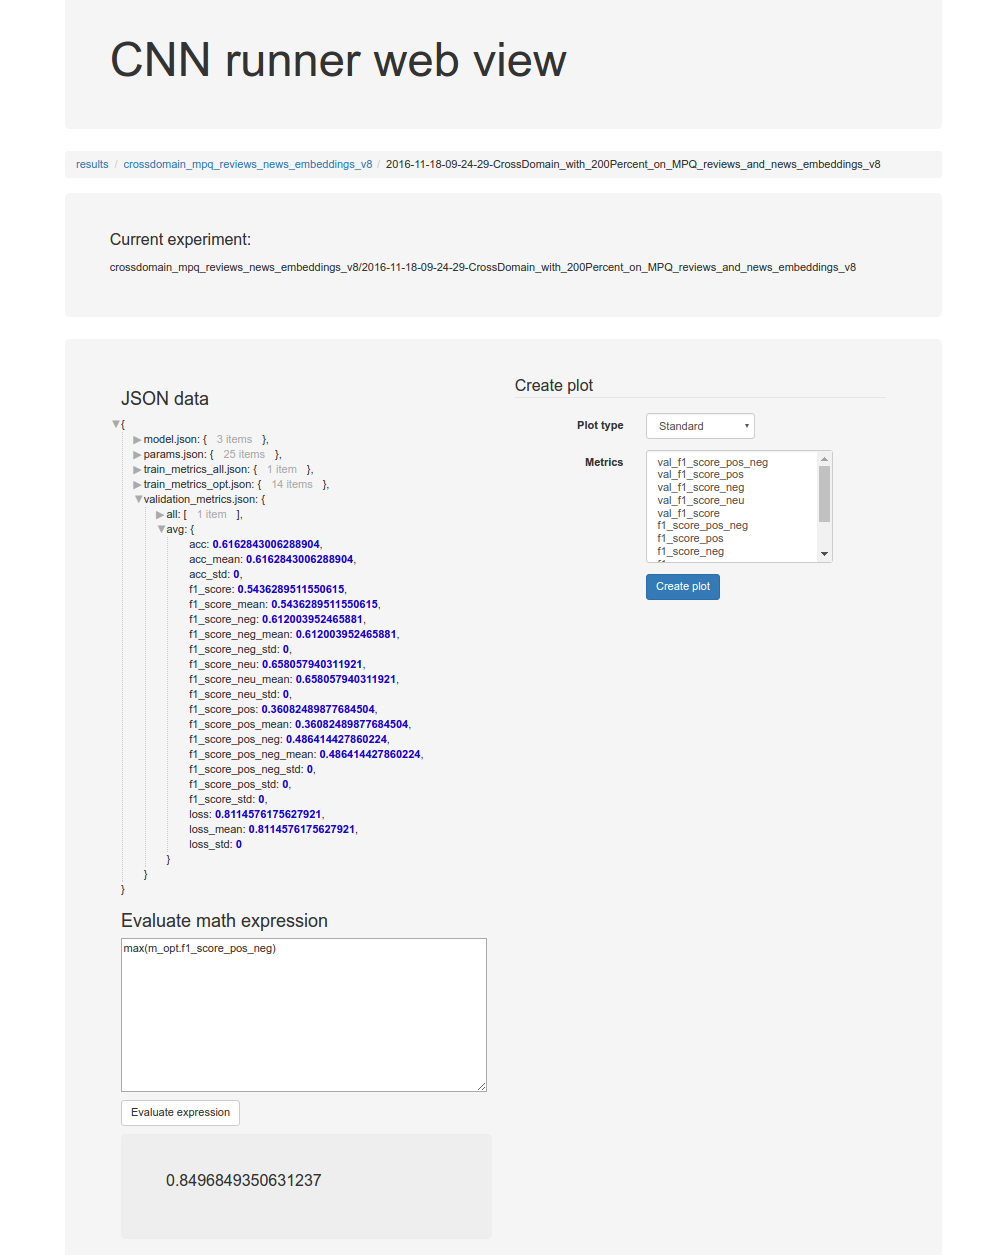
\includegraphics[width=0.7\textwidth]{img/web_gui}
	\caption{Ansicht Experiment über Weboberfläche}
	\label{fig:web_gui}
\end{figure}
\subsection{Betriebssystem \& Softwarepakete}
\label{technical_setup:software}
Alle Experimente wurden mit der unten beschriebenen Implementation durchgeführt. Auf beiden verwendeten Computer-Systemen (vgl. \ref{technichal_setup:prework}) wurde als Betriebssystem Ubuntu 16.04 installiert. Dazu wurden Python 3.5.2\footnote{https://www.python.org/}, Nvidia GPU Treiber und cuda8\footnote{https://developer.nvidia.com/cuda-toolkit} als Abhängigkeiten von Theano und Keras installiert.

\subsection{Hardware}
\label{technichal_setup:hardware}
Zur Durchführung der Experimente wurden zwei unterschiedliche Computer verwendet. Im ersten System (S1) ist eine Nvidia GTX970 GPU, einen Intel i7 4950K CPU und 16GB Arbeitsspeicher installiert. Das zweite System besitzt eine Nvidia GTX1070 GPU, einen Intel i7 6700K CPU und ebenfalls 16GB Arbeitsspeicher. Die Unterschiede in der Hardware haben keinen Einfluss auf die Experimente, da auf beiden System dasselbe Betriebssystem mit den gleichen Softwarepaketen verwendet wurde (vgl. \ref{technical_setup:software}).


\chapter{Daten}
Im  folgenden Kapitel werden die im Laufe dieser Arbeit verwendeten Trainingsdaten und Text Corpora genauer beschrieben. Es wird erläutert woher die Daten stammen, welchen Zweck sie erfüllen und wie die einzelnen Datensätze aufgebaut sind. Des Weiteren wird erläutert wie die Word-Embeddings und Datensätze für die Distant-Supervised Phase generiert werden.

Die Trainingsdaten, welche in dieser Arbeit verwendet werden, können in zwei Klassen unterteilt werden:

\begin{itemize}
	\item \emph{Supervised}: Datensätze, welche Texte und dazugehörige Sentiments mitliefern werden gehören zur Klasse der Supervised Datensätze. Dazu zählen beispielsweise alle Trainings- und Testdaten welche in den Folgenden Experimente verwendet werden.
	\item \emph{Unsupervised}: Datensätze, welche Texte aber keine zugehörigen Sentiments mitliefern gehören zur Klasse der Unsupervised Datensäte. Dazu zählen einerseits die Daten, mit welchen die Distant-Supervised Phase durchgeführt wird. Andererseits gehören hierzu auch die Text-Corpora mit welchen die Word-Embeddings generiert werden.
\end{itemize}

\clearpage

\subsection{Supervised}
\label{data:supervised_data}
Alle Datensätze welche während des Trainings und der Evaluierung eines \gls{CNN} verwendet werden liefern Texte und die dazugehörigen Sentiments mit. Da die Datensätze nur als ganzes zur Verfügung stehen werden diese von uns im Verhältnis 80\% Trainingsdaten und 20\% Testdaten zufällig unterteilt.
\paragraph{Trainingsdaten} Die in der folgenden Tabelle aufgelisteten Datensätze werden für das Training der \gls{CNN}s verwendet.
\begin{table}[H]
	\ra{1.3}
	\begin{adjustbox}{max width=\textwidth}
		\begin{tabular}{@{}lllcccccccl@{}}
			\toprule
			& & & & & & \multicolumn{3}{c}{Verteilung Sentiments} &\\
			\cmidrule(r){7-9}
			& Name & Textart & Anzahl Texte & \specialcell{Durchschnittliche\\Anzahl Zeichen} & \specialcell{Durchschnittliche\\Anzahl Wörter} & positiv & neutral & negativ & Quelle &\\ \midrule
			& DAI{\_}tweets & Tweets & $3274$ & $63.4$ & $16.1$ & $19.4\%$ & $66.9\%$ & $13.6\%$ & \cite{Narr:2012}\\
			& DIL{\_}reviews & Produktbewertungen & $3420$ & $74.0$ & $19.0$ & $31.1\%$ & $50.8\%$ & $17.9\%$ & \cite{Ding:2008}\\
			& HUL{\_}reviews & Produktbewertungen & $3156$ & $70.7$ & $18.6$ & $28.4\%$ & $57.7\%$ & $13.9\%$ & \cite{Hu:2004}\\
			& JCR{\_}quotations & Zitate aus Reden & $1032$ & $148.4$ & $33.6$ & $15.0\%$ & $71.3\%$ & $13.7\%$ & \cite{Balahur:2013}\\
			& MPQ{\_}news & Nachrichtentexte & $8888$ & $123.3$ & $26.9$ & $14.8\%$ & $55.5\%$ & $29.7\%$ & \cite{Wiebe:2005}\\
			& SEM{\_}headlines & Nachrichtenüberschriften & $1000$ & $34.3$ & $7.1$ & $14.4\%$ & $61.0\%$ & $24.6\%$ & \cite{Strapparava:2007}\\
			& SemEval{\_}tweets & Tweets & $8226$ & $89.1$ & $22.4$ & $37.2\%$ & $48.1\%$ & $14.7\%$ & \cite{SemEval:2016:task4}\\
			& TAC{\_}news & Nachrichtentexte & $2152$ & $88.6$ & $22.4$ & $36.3\%$ & $17.7\%$ & $46.0\%$ & \cite{Tackstrom:2011}\\
			\bottomrule
		\end{tabular}
	\end{adjustbox}
	\caption{Statistiken zu Texten der Trainingsdaten.}
\end{table}

\paragraph{Testdaten} Die in der folgenden Tabelle aufgelisteten Datensätze werden verwendet um die Performanz eines trainierten \gls{CNN} zu evaluieren.
\begin{table}[H]
	\ra{1.3}
	\begin{adjustbox}{max width=\textwidth}
		\begin{tabular}{@{}lllcccccccl@{}}
			\toprule
			& & & & & & \multicolumn{3}{c}{Verteilung Sentiments} &\\
			\cmidrule(r){7-9}
			& Name & Textart & Anzahl Texte & \specialcell{Durchschnittliche\\Anzahl Zeichen} & \specialcell{Durchschnittliche\\Anzahl Wörter} & positiv & neutral & negativ & Quelle &\\ \midrule
			& DAI{\_}tweets & Tweets & $819$ & $66.5$ & $16.8$ & $19.8\%$ & $67.9\%$ & $12.3\%$ & \cite{Narr:2012}\\
			& DIL{\_}reviews & Produktbewertungen & $855$ & $74.9$ & $19.2$ & $31.6\%$ & $51.6\%$ & $16.8\%$ & \cite{Ding:2008}\\
			& HUL{\_}reviews & Produktbewertungen & $789$ & $63.3$ & $17.1$ & $21.7\%$ & $53.3\%$ & $25.0\%$ & \cite{Hu:2004}\\
			& JCR{\_}quotations & Zitate aus Reden & $258$ & $143.6$ & $32.6$ & $14.7\%$ & $49.2\%$ & $36.1\%$ & \cite{Balahur:2013}\\
			& MPQ{\_}news & Nachrichtentexte & $2223$ & $121.6$ & $26.5$ & $13.1\%$ & $55.1\%$ & $31.8\%$ & \cite{Wiebe:2005}\\
			& SEM{\_}headlines & Nachrichtenüberschriften & $255$ & $33.4$ & $7.1$ & $12.0\%$ & $61.6\%$ & $26.4\%$ & \cite{Strapparava:2007}\\
			& SemEval{\_}tweets & Tweets & $3813$ & $89.6$ & $21.8$ & $41.2\%$ & $43.0\%$ & $15.8\%$ & \cite{SemEval:2016:task4}\\
			& TAC{\_}news & Nachrichtentexte & $537$ & $110.4$ & $26.7$ & $26.6\%$ & $12.1\%$ & $61.2\%$ & \cite{Tackstrom:2011}\\
			\bottomrule
		\end{tabular}
	\end{adjustbox}
	\caption{Statistiken zu Texten der Testdaten.}
\end{table}

\clearpage

\subsection{Unsupervised}
Im Folgenden werden die \emph{Unsupervised} Datensätze erläutert. Einerseits beinhalten diese die Text-Corpora mit welchen die Word-Embeddings generiert werden, andererseits gehören hierzu auch die Datensätze welche für das Training der \gls{CNN}s während der Distant-Supervised Phasen eingesetzt werden.

\paragraph{Text-Corpora} Im Rahmen dieser Arbeit werden vier verschiedene Arten von Word-Embeddings verwendet. Diese werden auf verschiedenen Text-Corpora generiert, welche in der folgenden Tabelle aufgelistet sind:

\begin{table}[H]
	\centering
	\ra{1.3}
	\begin{adjustbox}{max width=\textwidth}
		\begin{tabular}{@{}lllcccccccl@{}}
			\toprule
			Name & Beschreibung & Anzahl Sätze & Quelle\\ \midrule
			\emph{News} & News-Texte von diversen Webseiten & 90 Mio. & STATMT Webseite\tablefootnote{http://www.statmt.org/wmt14/training-monolingual-news-crawl/}\\
			\emph{Tweets} & Sammlung von öffentlich verfügbaren Tweets & 590 Mio. & Twitter-API\tablefootnote{https://dev.twitter.com/rest/public}\\
			\emph{Wiki} & Texte aller Artikel auf Wikipedia mit mehr als 50 Wörtern & 4.5 Mio. & Wikimedia\tablefootnote{https://dumps.wikimedia.org/enwiki/latest/}\\
			\bottomrule
		\end{tabular}
	\end{adjustbox}
	\caption{Text-Corpora, welche für die Generierung der Word-Embeddings verwendet werden.}
\end{table}
Zusätzlich werden während der Experimente zufällig initialisierte Word-Embeddings verwendet; diese werden im Folgenden mit \emph{Random} gekennzeichnet. Die Generierung der Word-Embeddings wurde mittels \emph{word2vec} \cite{mikolov2013distributed} durchgeführt. Dabei wurden die folgenden Hyperparameter verwendet:

\begin{table}[H]
	\centering
	\ra{1.3}
	\begin{adjustbox}{max width=\textwidth}
		\begin{tabular}{@{}lllcccccccl@{}}
			\toprule
			Name & Wert\\ \midrule
			\emph{algorithm} & skip-gram\\
			\emph{dimensions} & $52$\\
			\emph{window size} & $5$\\
			\emph{minimum count} & $15$\\
			\emph{sample} & $10^{-5}$\\
			\bottomrule
		\end{tabular}
	\end{adjustbox}
	\caption{Hyperparameter, welche für die Generierung der Word-Embeddings mit \emph{word2vec} verwendet werden.}
\end{table}

\clearpage

\paragraph{Datensätze für Distant-Supervised Phase} Im Rahmen dieser Arbeit werden zwei verschiedene Datensätze für die Distant-Supervised Phase verwendet: Produktbewertungen von Amazon\footnote{https://www.amazon.com/} und Kurznachrichtentexte von Twitter\footnote{https://twitter.com/}. Dabei werden die Sentiments bei den Produktbewertungen anhand der vergebenen Wertung und bei den Tweets anhand der im Text vorhandenen Emoticons abgeleitet. Bei den Produktbewertungen werden alle Texte, welche mit einer Wertung von $x >= 4$ als positiv, $x < 3$ als negativ klassifiziert; die Restlichen werden als neutral angenommen. Bei den Tweets wird ein Lexikon von positiven (z.B. \quotes{:-)}) und negativen (z.B. \quotes{:-(}) Emoticons verwendet. Dabei werden die positiven und negativen Emoticons im Tweet gezählt; die Klasse welche öfter vorhanden ist gibt den Sentiment des Tweets vor.\\\\
Dieses Schema führt zu folgenden Datensätzen, welche während der Distant-Supervised Phase verwendet werden:
\begin{table}[H]
	\ra{1.3}
	\begin{adjustbox}{max width=\textwidth}
		\begin{tabular}{@{}lllcccccccl@{}}
			\toprule
			& & & & & & \multicolumn{3}{c}{Verteilung Sentiments} &\\
			\cmidrule(r){7-9}
			& Name & Textart & Anzahl Texte & \specialcell{Durchschnittliche\\Anzahl Zeichen} & \specialcell{Durchschnittliche\\Anzahl Wörter} & positiv & neutral & negativ & Quelle &\\ \midrule
			& Amazon Reviews & Produktbewertungen & $82.4$ Mio. & $382.2$ & $96.2$ & $78.2\%$ & $8.5\%$ & $13.2\%$ & \cite{Zhang:2015}\\
			& Tweets & Tweets & $100.0$ Mio. & $46.9$ & $12.4$ & $79.1\%$ & $0.0\%$ & $20.9\%$ & Twitter-API\tablefootnote{https://dev.twitter.com/rest/public}\\
			\bottomrule
		\end{tabular}
	\end{adjustbox}
	\caption{Statistiken zu Texten der Distant-Supervised Datensätze.}
\end{table}

Des Weiteren werden auch Experimente ohne Distant-Supervised Phase durchgeführt; diese werden mit \emph{None} gekennzeichnet.

\chapter{Methoden}
In diesem Kapitel wird aufgezeigt, wie die im Kapitel Einführung genannten Fragestellungen untersucht wurden.\\\\
Der Kern dieser Arbeit dreht sich um folgende Frage: Verbessert sich ein CNN für eine spezifische Domäne, durch das hinzufügen domänenfremder Daten während der supervised Phase.
\section{F1 Score}
Um die Ergebnisse der Experimente zu vergleichen, wurde der positive und negative gemittelte F1 Score gewählt.
Der F1 Score wird folgendermassen berechnet:\\
\begin{equation}
F1 = 2*\frac{precission*recall}{precission+recalll}
\end{equation}\\
Der F1 Score wird für die positiven, wie auch die negativen Fälle berechnet und dann wie folgt gemittelt:\\
\begin{equation}
F1_{pn} = \frac{F1_p+F1_n}{2}
\end{equation}\\
Dieser Wert gilt als Standart, um die Qualität binärer Klassifizierung zu messen. Der grosse Vorteil dieses Masses ist, dass durch eine einseitige, falsche Klassifizierung, der Wert sehr schlecht wird.
\section{Word-Embeddings und Distant-Phase}
\subsection{Word-Embeddings}
Alle beschriebenen Experimente wurden mit 2 verschiedenen Word-Embeddings durchgeführt. Dabei soll der Einfluss, vielleicht auch eine Korrelation, zwischen den gewählten Word-Embedings und der Zieldomäne untersucht werden. Die Experimente wurden mit Tweets und News Embeddings durchgeführt. Dass Tweets häufig aus vielen kurzen, teilweise auch stark abgekürzte, Sätzen bestehen und News aus längeren, grammatikalisch korrekten Sätzen, wurde absichtlich so gewählt, damit der Unterschiede im Resultat gut ersichtlich währen.
\subsection{Distant-Phase}
Aus der Arbeit \cite{deriu2016sentiment} ist ersichtlich, dass dieser Vorgang mit Tweets eine Verbesserung von fast 5 Prozentpunkte auf den $F1_{pn}$ Score erbrachte.
Deshalb wurde in dieser Arbeit eine Distant-Phase auf Reviews getestet. Alle nachfolgend beschrieben Experimente wurden einmal mit und einmal ohne einer Distanz-Phase auf Amazon Reviews durchgeführt.

\section{Aufbau der Experimente}
Die folgenden Experimente wurden jeweils für die Zieldomäne SemEval Tweets und MPQ Reviews durchgeführt. Bei allen Experimenten wird das CNN mit den gleichen Parametern initialisiert. Zusätzlich wurden alle Experimente drei Mal ausgeführt, um eine allfällige Varianz auszuschliessen.
\subsection{Experiment V6}
Mit dem Experiment V6 wurde die Kernfrage untersucht, ob die Performanz eines CNN steigt, wenn Domänenfremde Daten in die Trainingsphase mit einbezogen werden.
In einem ersten Schritt wurde das CNN mit domänenfremden Daten trainiert. Anschliessend wird das CNN in 20 Einzelschritten zusätzlich mit Daten von der Zieldomäne weiter trainiert. Die genaue Aufteilung auf die verschiedenen Domänen ist im Bild \ref{fig:Method_V6} ersichtlich.
\begin{figure}[htbp]
	\centering
	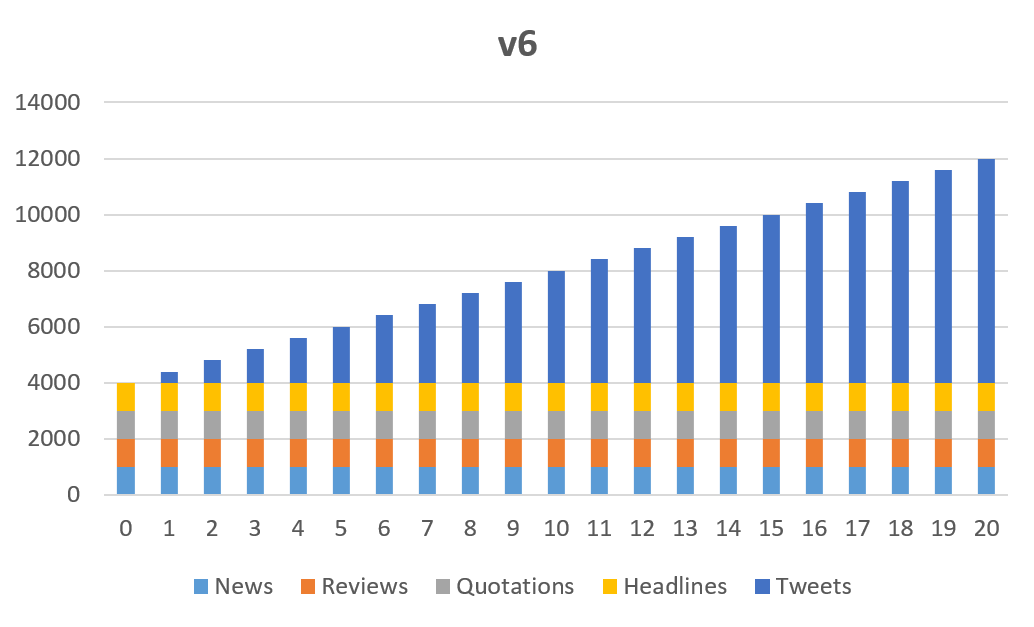
\includegraphics[width=0.7\textwidth]{img/Method_V6}
	\caption{Aufbau Experiment V6 - Tweets}
	\label{fig:Method_V6}
\end{figure}
Bei \ref{fig:Method_V6} ist die Zieldomäne SemEval Tweets, die Vorgehensweise für die Zieldomäne MPQ Reviews unterscheidet sich nicht.
\subsection{Experiment V7}
Im Experiment V7 wurde untersucht, wie stark sich die Performanz eines bereits trainierten CNN verbessert, wenn mit der Zieldomäne ähnlichen Daten weiter trainiert wird. Konkret bedeuted dies, es wird ein CNN für die Zieldomäne MPQ Reviews trainiert. Anschliessend wird in 10 Teilschritten mit einer steigenden Anzahl anderer Review Domänen (siehe Kapitel Daten), weiter trainiert.
%TODO Kapitel Date referenzieren?
%TODO insert Picture

\subsection{Experiment V8}
Das Experiment V8 dient als Baseline und somit Referenzwert für die Experimente V6 und V7.
Bei diesem Experiment wird nur mit den Daten der Zieldomäne trainiert und validiert \ref{fig:Method_V8}. Es dient als Anhaltspunkt, ob die Idee CrossDomain eine effektive  Steigerung der Performanz erbringen kann.
\begin{figure}[htbp]
	\centering
	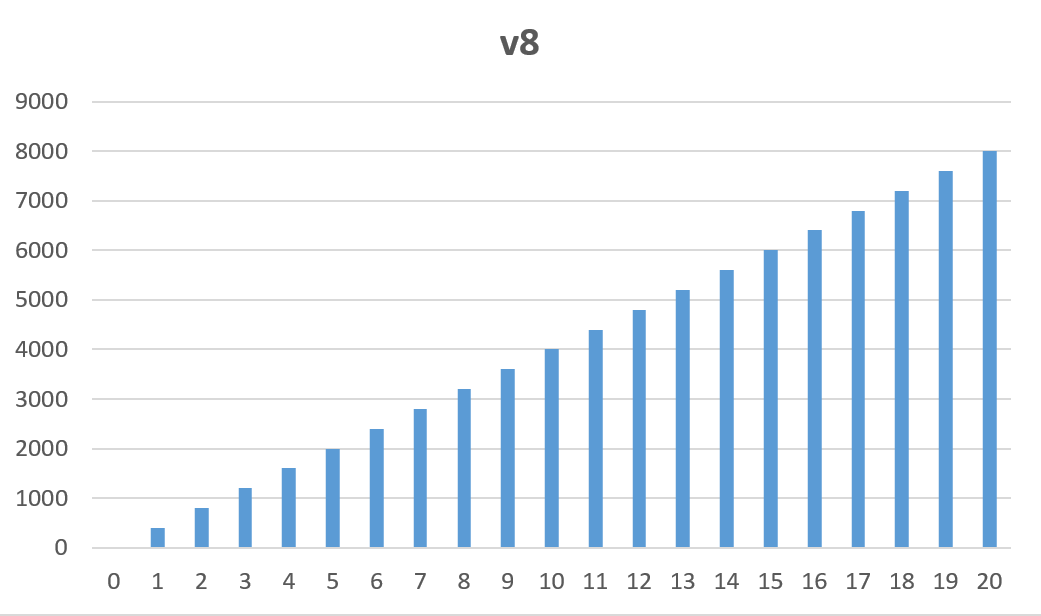
\includegraphics[width=0.7\textwidth]{img/Method_V8}
	\caption{Aufbau Experiment V8}
	\label{fig:Method_V8}
\end{figure}
%TODO CrossDomain in Glossar
$TODO F1_{pn} in Glossar 

\chapter{Resultate}
RESULTS
\chapter{Interpretation}
INTERPRETATION
\chapter{Schlussfolgerungen}
CONCLUSION
\chapter{Ähnliche Arbeiten}
RELATED WORK
\chapter{Referenzen}
\begin{thebibliography}{9}
  
  \bibitem{SwissCheeseSemEval}
  F. Hess. (25.05.2015). \emph{Alkoholrechner - Android-Apps auf Google Play} [Online]. URL: \url{https://play.google.com/store/apps/details?id=appinventor.ai_fabrice_hess1999.Alkoholrechner}

\end{thebibliography}
\glsaddall
\glossarystyle{altlistgroup}
\printglossary[title=Glossar]
\appendix

\listoftables
\listoffigures

\end{document}
